%-Define the offline and two trigger clusters
%-explain difference between two trigger level clusters
%-Show the matching cuts
%-Explain the reason for the plots
%-For the plot, make sure we explain the red points.

The EM calorimeter component of the HLTCalo is monitored by using physics objects that are reconstructed using EM energy deposits from electrons and photons. 
There are differences between the L2 and EF level EM cluster finding due to the time constraints on the L2 trigger.  
The L2 EM clusters are found using only the second EM calorimeter layer, in which the highest energy cell is used as the cluster seed.
From this cluster seed, the cluster position is formed using the energy weighted $\eta$ $\phi$ from a grid \etaphi{0.075} around the seed and the cluster energy is calculated by summing over the energy of the cells. 
Conversely, the EF EM clusters use a sliding window cluster algorithm using the calo towers. 
This reduces the effect of the hot cells, as these will be smeared by the surrounding regular cells which will not have energy deposits.
The offline cluster are also found using a sliding window algorithm, but have full offline cell information.
 

\subsubsection{EM cluster matching}

Matching the offline and trigger objects is done using a \dr{} cut.

Figure \ref{SW_egamma_L2_dR} is the \dr{} distribution between the offline and all L2 EM cluster.
There is two peaks that can be seen in (a), one at $\dr{}=0$ which corresponds to good matching.
Events often have two objects that will be back-to-back in \dphi{}, which corresponds to the peak at $\dr{}\approx3$. 
The peak at $\dr{}=0$ is better seen in (b), and shows a minimum in the range \dr{} of 0.03 to 0.1.

Figure \ref{SW_egamma_EF_dR} is the \dr{} distribution between the offline and all EF EM cluster.
As observed for the L2 \dr{} distribution, there are two peaks at $\dr{}=0$ and $\dr{}\approx3$. 
The minimum observed in (b) is in the range \dr{} of 0.02 to 0.1.

A \dr{} matching cut of 0.035 is used for both L2 and EF as this selects the majority of the correctly matched clusters and is also the distance from the centre to the edge of the L2 cluster.
Additionally the offline cluster is required to have a $\et{}>10$ GeV.  

\begin{figure}
\centering
\mbox{
   \subfigure[]{\epsfig{figure=figures/ServiceWork/EgammaL2/DR_Unmatched_L2.eps,width=0.5\textwidth}}\quad
      \subfigure[]{\epsfig{figure=figures/ServiceWork/EgammaL2/DR_Unmatched_Zoomed_L2.eps,width=0.5\textwidth}}\quad
}
\caption[\dr{} between offline and L2 egamma object]{\dr{} between the offline egamma cluster and all L2 clusters in the event, shown with range (a) $0 - 5$ and (b) $0 - 0.3$ \label{SW_egamma_L2_dR}}
\end{figure}

\begin{figure}
\centering
\mbox{
   \subfigure[]{\epsfig{figure=figures/ServiceWork/EgammaEF/DR_Unmatched_EF.eps,width=0.5\textwidth}}\quad
      \subfigure[]{\epsfig{figure=figures/ServiceWork/EgammaEF/DR_Unmatched_Zoomed_EF.eps,width=0.5\textwidth}}\quad
}
\caption[\dr{} between offline and EF egamma object]{\dr{} between the offline egamma cluster and all EF clusters in the event, shown with range (a) $0 - 5$ and (b) $0 - 0.3$\label{SW_egamma_EF_dR}}
\end{figure}




\subsubsection{Monitored Distributions}


The monitoring plots shown in Figures \ref{SW_egamma_L2EF_EtEt} -\ref{SW_egamma_L2EF_Reso} are from run 190644 in the  2011 data-taking.


Figure \ref{SW_egamma_L2EF_EtEt} shows the distribution of the offline EM cluster \et{} to that of (a) L2 and (b) EF EM cluster \et{}.
This is useful in checking the linearity of the trigger EM clusters to the offline. 
Th L2 EM cluster \et{} shows good linearity to the offline EM cluster \et{}, and the majority of events fall on a straight line where the \et{} of the offline and L2 are the same.
There is a significant band either side of this straight line, with more falling above the line, which corresponds to a larger offline than L2 EM cluster \et{}.
The EF EM cluster \et{} has an even better linearity, and again most of events falling on a straight line corresponding to the offline EF clusters having the same \et{}.
The band around the events falling on the straight line is significantly smaller than for the L2 EM clusters.


Figure \ref{SW_egamma_L2EF_EtFrac} shows the distribution of \et{} fraction,
\begin{equation}
f(\et{})_{Trigger}=\frac{\et{}(\rm{Triggered~EM~cluster})}{\et{}(\rm{Offline~EM~cluster})},
\label{SW:EtFrac}
\end{equation}
as a function of $\eta{}$ for (a) the L2 EM clusters and (b) EF EM clusters.
The \et{} fraction for the L2 EM clusters is centred around one, with most events within $5\%$.
The EF EM clusters \et{} fraction is also centred around one, but with significantly smaller fluctuations.
In both the distributions there is a region at $|\eta{}|=1.5$ where the fluctuations from one are larger.
This is due to the EM deposit falling into the crack region between the EM calorimeter barrel and the EM barrel end-cap.
There is an improvement in the EF due to the additional calibration done at EF level. 

Figure \ref{SW_egamma_L2EF_Reso} shows the distribution of the \et{} resolution,
\begin{equation}
Reso_{Trigger}=\frac{\et{}(\rm{Triggered~EM~cluster})-\et{}(\rm{Offline~EM~cluster})}{\et{}(\rm{Offline~EM~cluster})},
\label{SW:EtReso}
\end{equation}
for (a) L2 EM clusters and (b) EF EM clusters.
Both distributions show a mean \et{} distribution within a percent of zero. 
The L2 EM clusters \et{} resolution distribution has a larger spread than the EF.


All the monitoring distributions are susceptible to changes in calibration or the cluster sizes, which are changed occasionally. 
The monitoring flags can be set for a distribution to compare the mean of the distribution to the expected.
The distributions in Figures \ref{SW_egamma_L2EF_EtFrac} and \ref{SW_egamma_L2EF_Reso} have flags set based on the mean of the \et{} fraction and \et{} resolution respectively. 
If these show sizable differences from the expected mean, the distribution will be yellow or red flagged automatically.
Figure \ref{SW_egamma_L2EF_EtEt} can then be used to study the reason for the differences.

 
\begin{figure}
\centering
\mbox{
   \subfigure[]{\epsfig{figure=figures/ServiceWork/run_190644/EtEt_Matched_L2.eps,width=0.5\textwidth}}\quad
      \subfigure[]{\epsfig{figure=figures/ServiceWork/run_190644/EtEt_Matched_EF.eps,width=0.5\textwidth}}\quad
}
\caption[Offline egamma \et{} versus L2 and EF egamma \et{}]{\et{} of the offline egamma cluster versus the \et{} of the closest matched (a) L2 and (b) EF egamma cluster.\label{SW_egamma_L2EF_EtEt}}
\end{figure}

\begin{figure}
\centering
\mbox{
   \subfigure[]{\epsfig{figure=figures/ServiceWork/run_190644/EtFrac_Eta_Matched_L2.eps,width=0.5\textwidth}}\quad
      \subfigure[]{\epsfig{figure=figures/ServiceWork/run_190644/EtFrac_Eta_Matched_EF.eps,width=0.5\textwidth}}\quad
}
\caption[\et{} fraction of L2 and EF to offline egamma objects]{\et{} fraction of the (a) L2 and (b) EF egamma cluster to the offline egamma cluster \et{} as a function of $\eta$. \label{SW_egamma_L2EF_EtFrac}}
\end{figure}

\begin{figure}
\centering
\mbox{
   \subfigure[]{\epsfig{figure=figures/ServiceWork/run_190644/Reso_Matched_L2.eps,width=0.5\textwidth}}\quad
      \subfigure[]{\epsfig{figure=figures/ServiceWork/run_190644/Reso_Matched_EF.eps,width=0.5\textwidth}}\quad
}
\caption[Offline egamma \et{} versus L2/EF egamma \et{}]{Percentage difference of the (a) L2 and (b) EF egamma cluster \et{} to the offline egamma cluster \et{}\label{SW_egamma_L2EF_Reso}}
\end{figure}


Figure \ref{SW_egamma_EF_Reso_Range} is the history of the mean of \et{} resolution for EF egamma clusters.
The colours of the points show the flag that was set for these runs.
Flags were assigned for a given run depending on the difference of the mean to a standard mean of $0.975\%$. 
The run is flagged green if the difference is less than $0.2\%$, yellow if between $0.2\% - 0.4\%$ or red if greater than $0.4\%$.
These flag values were tuned using the initial runs in the first data taking region.
Most of the runs are set as green or yellow, with only a few set as red.
The red flagged runs are runs where there is no stable beam and there are problems with the LAr calorimeter caused by *****  There is a problem here, just following up with Denis to find out what it is*****

\begin{figure}
\centering
\mbox{
   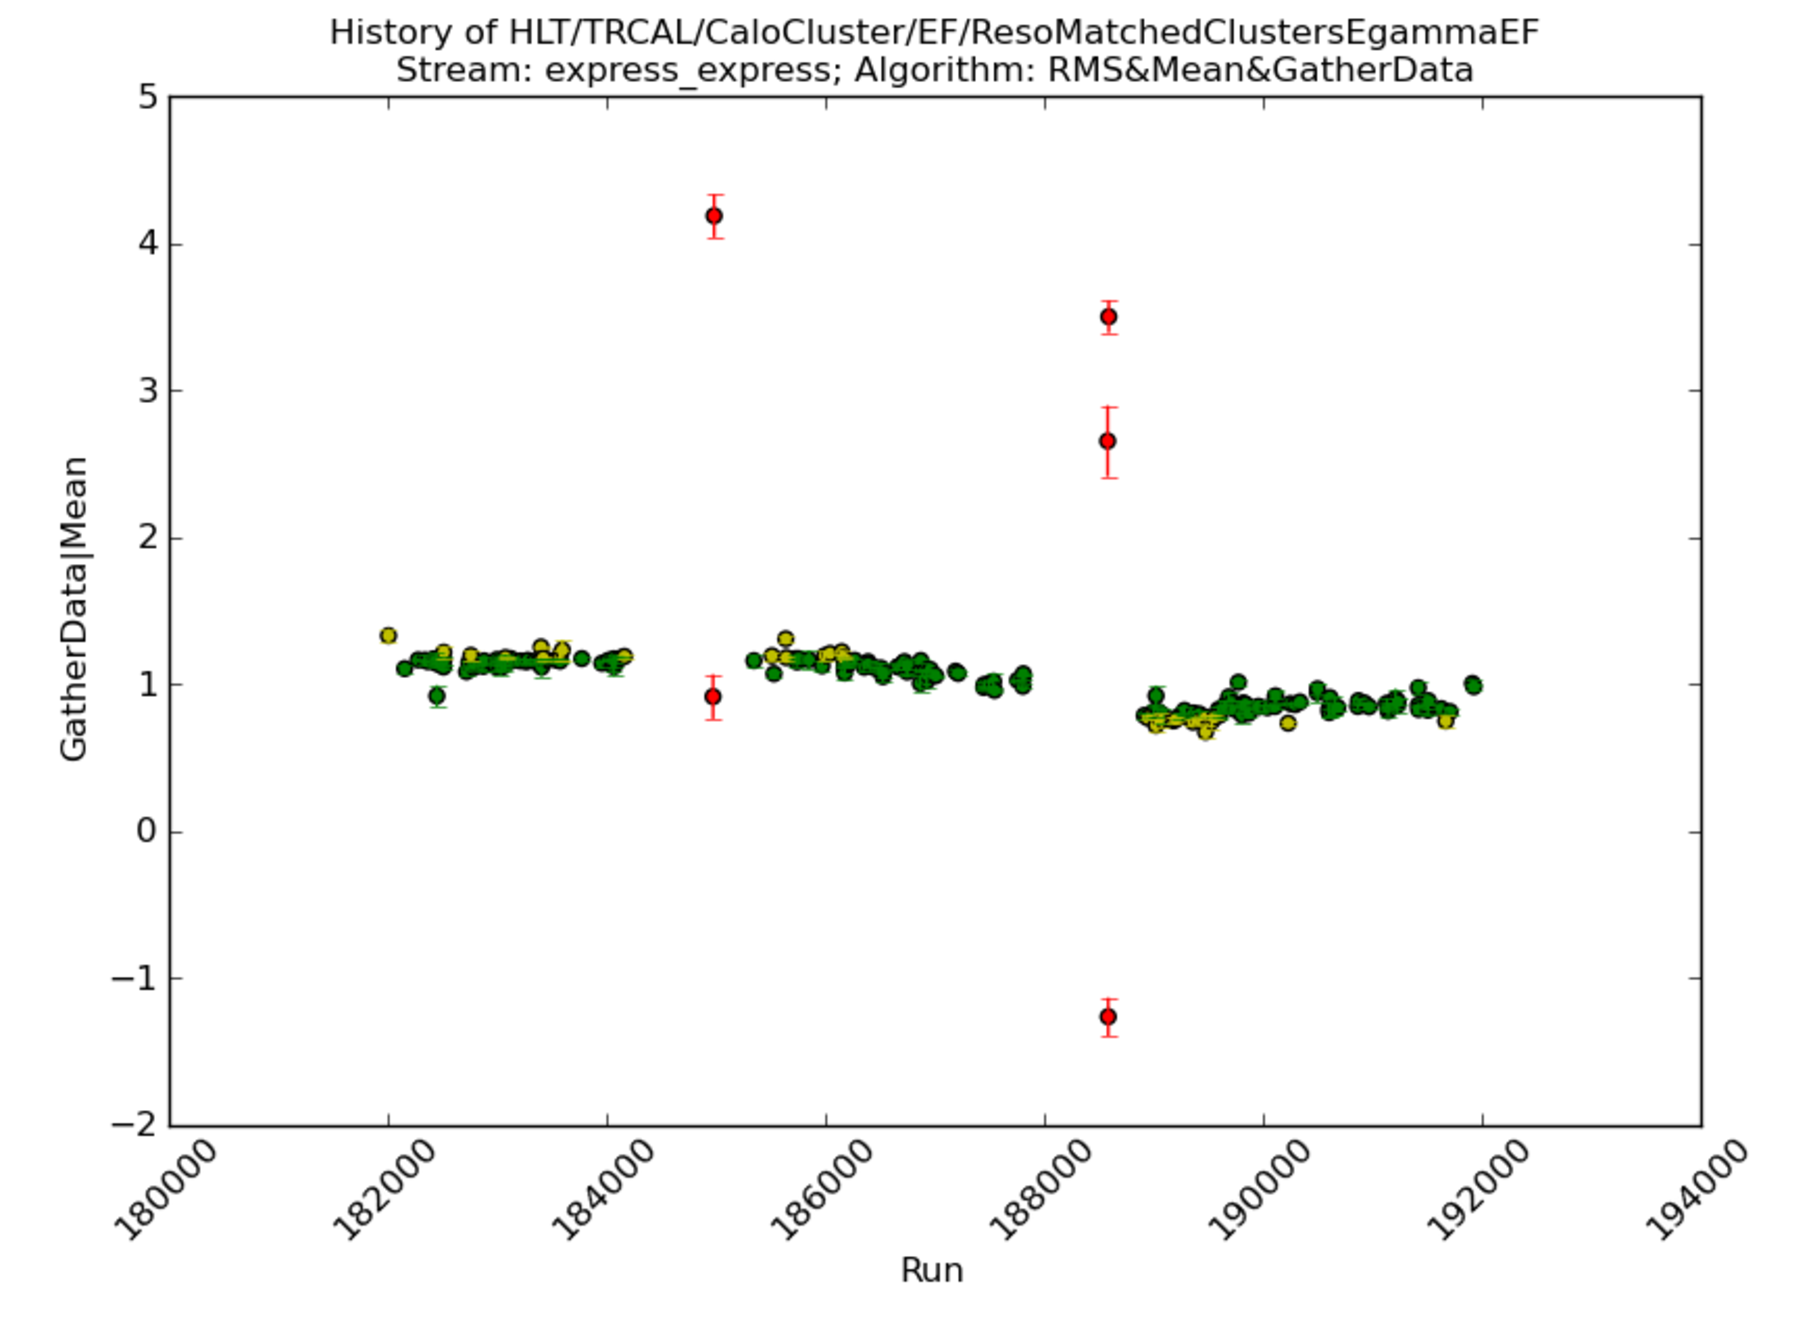
\includegraphics[width=1.0\textwidth]{figures/ServiceWork/EF_Reso_Range.pdf}
}
\caption[Offline egamma \et{} versus L2/EF egamma \et{}]{Mean of Figure \ref{SW_egamma_L2EF_Reso} (b) as a function of run number. \label{SW_egamma_EF_Reso_Range}}
\end{figure}

